\subsection{Reinforcement Learning}
\label{sec::323_rl}
The goal in reinforcement learning is not only to learn actions $A_t$, given a state $S_t$, like it is in behavioral cloning, but further to explore actions and states. This is usually performed as shown in figure \ref{fig::323_rl}, where an agent interacts with an environment to receive a reward $R_t$, and also changes the state as cause of its action. The difficulty therein is to have an agent to discard immediate rewards over future expected rewards, and it got first solved by deep Q-learning \cite{mnih2015human}, although it works best for discrete actions spaces. Different approaches for continuous action spaces like trust region policy optimization \cite{schulman2015trust} are rather complicated. The, to this date, most elegant way of solving continuous control problems in a reinforcement learning setup is proximal policy optimization \cite{schulman2017proximal}, and we will elaborate on it in the following. 




\cite{schulman2015high}



\begin{figure}[h]
	\centering
	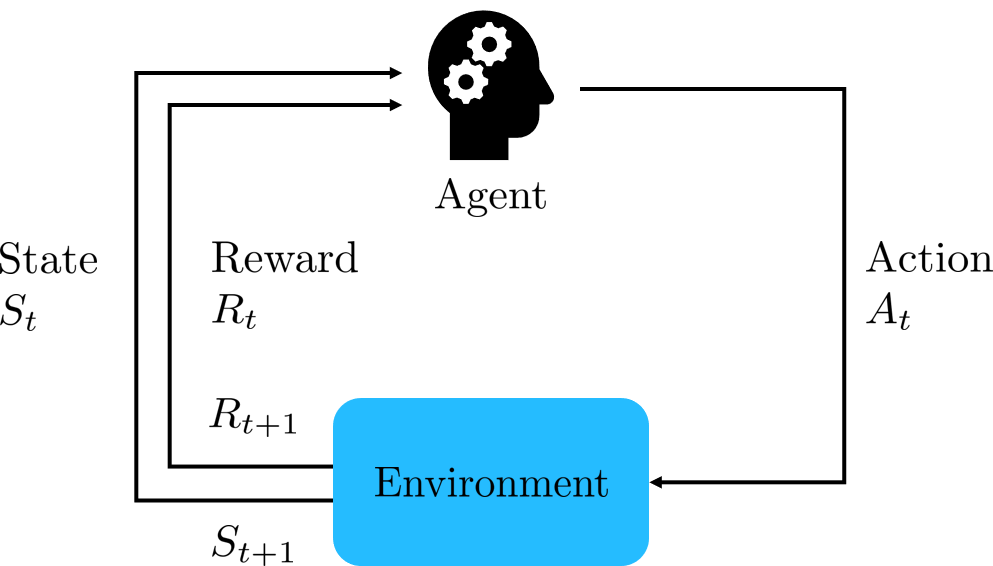
\includegraphics[scale=.5]{chapters/03_background/img/reinforcement_learning.png}
	\caption{Reinforcement learning setup.}
	\label{fig::323_rl}
\end{figure}
\begin{figure}[h]
	\centering
	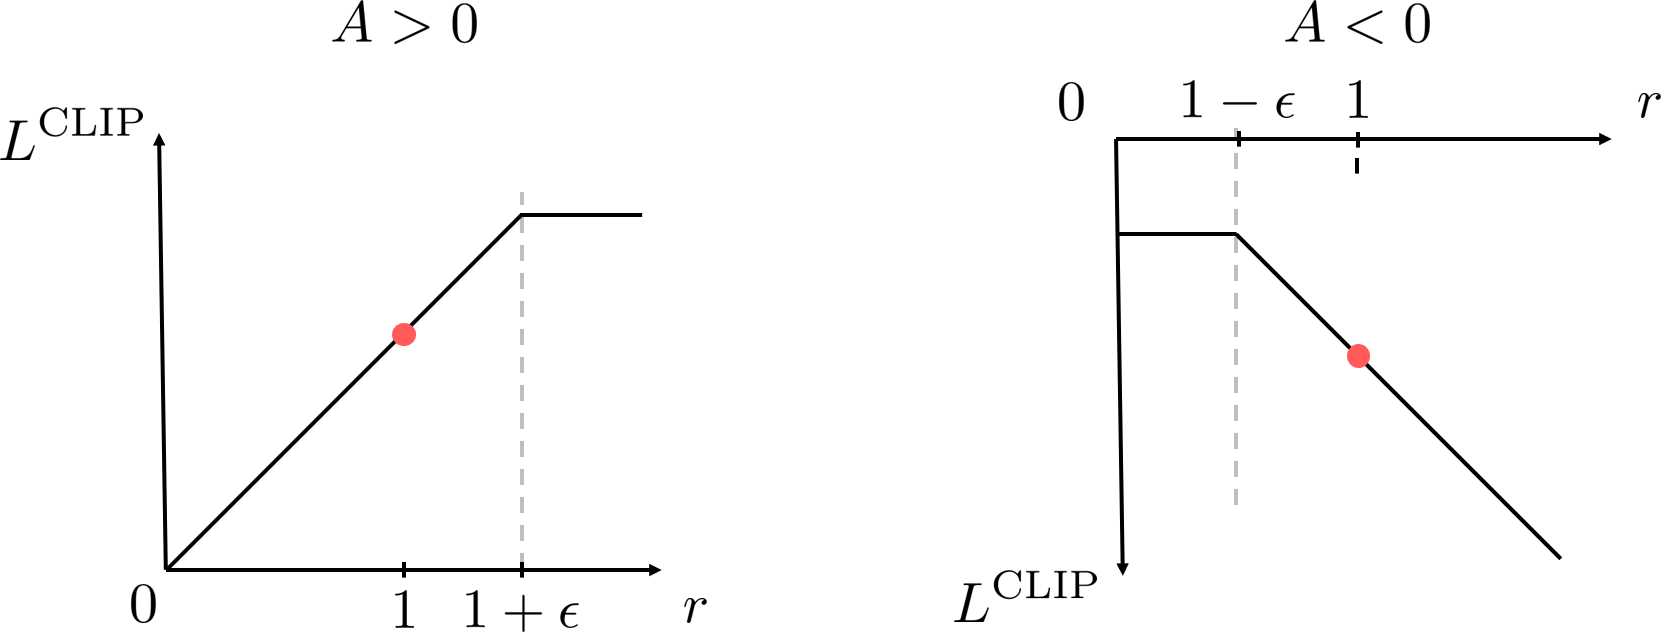
\includegraphics[scale=.35]{chapters/03_background/img/ppo_objective.png}
	\caption{PPO}
	\label{fig::323_ppo}
\end{figure}